\documentclass[12pt,phd,times]{pkmthesis}

\usepackage{amsmath,epsfig,graphicx,setspace,url,float}
\usepackage{pstricks,colortab,pifont}
\usepackage{lscape,multicol,multirow,longtable,subfigure}
\usepackage{cite, bm}   
\usepackage{geometry}
\usepackage{array}
\usepackage{algorithm}
\usepackage{multirow}
\usepackage{tabularx}
\usepackage{graphicx} 
\usepackage{subcaption}
\usepackage{booktabs}% Due to this hyberref will not work for references (PKM on 07/07/08)
\usepackage{tikz}
\usetikzlibrary{shapes.geometric, arrows, positioning, fit, backgrounds, decorations.pathreplacing}
\usepackage{cite}
\usepackage[english]{babel}
\usepackage[font=small,labelfont=bf]{caption}              % Added on 26/08/08
%\usepackage{slashbox} 
\usepackage{csquotes}  
\usepackage{threeparttable}
%\usepackage{adjustbox}                    % Added on 24/10/08 (Senthil)
\setlength{\textfloatsep}{1cm}              % Spacing b/w  float and text (PKM 01/11/08)
%..........................................................................................................................................
\normalem                                   % Added on 01/07/08 to avoid underline in the references
\setlength{\abovecaptionskip}{8pt}          % Added on 08/07/08
\setlength{\belowcaptionskip}{8pt}          % Added on 08/07/08
%..........................................................................................................................................
\usepackage{hyperref}
\usepackage{extra_functions}
%\input{pagesetup_pkm_twoside.tex}           % Modified on 06/07/08, 10/07/08, 15/07/08
%\input{pagesetup_pkm_singleside.tex}       % For Single Sided Document 
\input{pagesetup_pkm_middleside.tex}       % Middle alignment 
\raggedbottom                               % o6/08/08  (Remove Unnecessary space b/w paragraphs)
%******************************************************************************************************************************************

\begin {document}
\setcounter{page}{1} \pagenumbering{roman}  % 03/07/08
\doublespacing                              % or use \baselineskip 12pt (12, 18 and 24)
%*************************************************** FRONT PAGES**********************************************
%\thispagestyle{empty}
%\pdfbookmark{Title}{Title}
%\begin{center}
\fontsize{15.8pt}{19pt}\selectfont
{\textbf{Next-Day Hourly Stockout Prediction for Fresh Retail Supply Chains \\}}
\vspace*{0.13in}
\emph{\large{A report submitted in fulfillment for the award of the degree of}} \\
\emph{\large{Bachelors of Technology \\}}
\large{in \\}
\large{Information Technology\\}
\large{Bachelors of Technology Project \\}
\large{\textbf{Final Evaluation Report}}

\large{By}\\
 \large{\textbf{Anurag Thakur 2023IMG-008}} \\
 \large{\textbf{Samyak Choudhary 2023IMG-044}} \\
 \large{\textbf{Vibhor Kumar 2023IMG-054}} \\
\large{Under the Supervision of} \\
 \large{\textbf{Dr. Sunil Kumar}} \\
\large{Department of Information Technology}
\end{center}
\begin{figure}[!h]
\centerline{\includegraphics*[width = 3cm]{FrontPages/ABV_IIITM_logo.eps}}
%\centerline{
\epsfig{figure=FrontPages/thapar_logo.eps, []}}
%\centerline{\epsfig{figure=FrontPages/iitg.eps,scale=0.6}}
\end{figure}
\centerline {\large{ABV-INDIAN INSTITUTE OF INFORMATION TECHNOLOGY }}
\centerline{\large{AND MANAGEMENT GWALIOR}} \vspace*{0.05in}
\centerline{\large{GWALIOR, INDIA}} \vspace*{0.05in}
%\centerline{\large{DECEMBER, 2022.}}

%\thispagestyle{empty}
%\clearpage

\thispagestyle{empty}
\pdfbookmark{Title}{Title}
\begin{center}
\fontsize{15.8pt}{19pt}\selectfont
{\textbf{Next-Day Hourly Stockout Prediction for Fresh Retail Supply Chains \\}}
\vspace*{0.13in}
\emph{\large{A report submitted in fulfillment for the award of the degree of}} \\
\emph{\large{Bachelors of Technology \\}}
\large{in \\}
\large{Information Technology\\}
\large{Bachelors of Technology Project \\}
\large{\textbf{Final Evaluation Report}}

\large{By}\\
 \large{\textbf{Anurag Thakur 2023IMG-008}} \\
 \large{\textbf{Samyak Choudhary 2023IMG-044}} \\
 \large{\textbf{Vibhor Kumar 2023IMG-054}} \\
\large{Under the Supervision of} \\
 \large{\textbf{Dr. Sunil Kumar}} \\
\large{Department of Information Technology}
\end{center}
\begin{figure}[!h]
\centerline{\includegraphics*[width = 3cm]{FrontPages/ABV_IIITM_logo.eps}}
%\centerline{
\epsfig{figure=FrontPages/thapar_logo.eps, []}}
%\centerline{\epsfig{figure=FrontPages/iitg.eps,scale=0.6}}
\end{figure}
\centerline {\large{ABV-INDIAN INSTITUTE OF INFORMATION TECHNOLOGY }}
\centerline{\large{AND MANAGEMENT GWALIOR}} \vspace*{0.05in}
\centerline{\large{GWALIOR, INDIA}} \vspace*{0.05in}
%\centerline{\large{DECEMBER, 2022.}}

\thispagestyle{empty}

\clearpage
\thispagestyle{empty}
\pdfbookmark{Dedication}{Dedication}
%\include{FrontPages/Dedication}
\newpage
\thispagestyle{empty}
\clearpage
\thispagestyle{empty}
\pdfbookmark{Certificate}{Certificate}
\include{FrontPages/Certificate}
\newpage
\thispagestyle{empty}
\clearpage

\thispagestyle{empty}
\pdfbookmark{Acknowledgement}{Acknowledgement}
%\begin{acknowledgments}
\begin{center}
{\LARGE \bf Acknowledgements}
\end{center}
\begin{flushright}
\textit{\textbf{Name}}
\end{flushright}



%\end{acknowledgments}

\thispagestyle{empty}
\clearpage

\thispagestyle{empty}
%\pdfbookmark{Abstract}{Abstract}
%\renewcommand{\baselinestretch}{1.1}
%\include{FrontPages/Abstract2}
{\renewcommand{\baselinestretch}{1.5}
{%\small\normalsize
\begin{center}
	{\bf{Abstract}}
\end{center}
{\em{\noindent 
This project addresses the critical challenge of high-frequency intra-day stockouts in fresh retail supply chains, a domain where traditional daily-aggregated forecasting often fails. Utilizing the FreshRetailNet-50K dataset, we shifted from broad supply/backorder research to granular, store-level hourly predictions. We progressed from initial PyTorch Tabular baselines to standard recurrent models (Vanilla RNN and LSTM), establishing a foundation for explicitly handling chronological dependencies. Through rigorous architectural ablation, we engineered the Dual-Stream Inventory Shortcut LSTM, a custom architecture that processes demand and inventory signals independently while bypassing recurrent bottlenecks to route the latest inventory data directly to the output. Finally, in a standardized benchmarking framework incorporating threshold scanning and Focal Loss, we identified the Multi-Kernel DLinear (Decomposition Linear) architecture as our concluding state-of-the-art model. By capturing both short-term volatility and longer-term trends with remarkable parameter efficiency (13K parameters), the Multi-Kernel DLinear achieved a peak Hour-Level F1-Score of 0.8131, providing a highly deployable, interpretable solution for proactive shelf replenishment.
% \par    

	}}}}	
\thispagestyle{empty}
\clearpage

%..........................................................................................................................................
% For the fancy chapters (Don't remove these lines- 03/07/08)
\clearpage
\thispagestyle{empty}
\dominitoc
\dominilof
\dominilot
\fancyhf{} \fancyhead[LE]{\bfseries\small{\leftmark}}
\fancyhead[RO]{\bfseries\small{\rightmark}}
\fancyfoot[CE,CO]{\bfseries\thepage}
%..........................................................................................................................................
%TABLE OF CONTENTS
\renewcommand{\baselinestretch}{1}
\pdfbookmark[0]{Index}{index}
\pdfbookmark[1]{Contents}{toc}
\fancyhead[LE]{\bfseries\small{Contents}}
\fancyhead[RO]{\bfseries\small{Contents}}
\tableofcontents
\clearpage
%.........................................................................................................................................
 %LIST OF FIGURES
\pdfbookmark[1]{List of Figures}{lof}
\addstarredchapter{List of Figures}       % PKM 05/07/08 (For more options  refer minitoc.pdf on page 36)
\fancyhead[LE]{\bfseries\small{List of Figures}}
\fancyhead[RO]{\bfseries\small{List of Figures}}
\listoffigures
\clearpage
%..........................................................................................................................................
% LIST OF TABLES
\pdfbookmark[1]{List of Tables}{lot}
\addstarredchapter{List of Tables}         % or use \mtcaddchapter[List of Tables] [Please Refer minitoc.pdf]
\fancyhead[LE]{\bfseries\small{List of Tables}}
\fancyhead[RO]{\bfseries\small{List of Tables}}
\listoftables
\clearpage
%..........................................................................................................................................
% LIST OF ACRONYMS
\fancyhead[LE]{\bfseries\small{List of Acronyms}}
\fancyhead[RO]{\bfseries\small{List of Acronyms}}
%\pdfbookmark[1]{List of Acronyms}{loa}
%\addstarredchapter{List of Acronyms}
%\include{FrontPages/Acronyms}
\clearpage
%..........................................................................................................................................
% LIST OF SYMBOLS
\fancyhead[LE]{\bfseries\small{List of Symbols}}
\fancyhead[RO]{\bfseries\small{List of Symbols}}
%\pdfbookmark[1]{List of Symbols}{los}
%\addstarredchapter{List of Symbols}
%\include{FrontPages/Symbols}
\clearpage
%..........................................................................................................................................
\fancyhf{}
\fancyhead[LE]{\bfseries\small{\leftmark}}
\fancyhead[RO]{\bfseries\small{\rightmark}}
\fancyfoot[CE,CO]{\bfseries\thepage}
\setcounter{page}{1} \pagenumbering{arabic}
\renewcommand{\labelenumi}{(\roman{enumi})}   % Added on 09/08/2008
%*******************************************************************************************************************************************************************************************


%************************************************ BEGIN CHAPTERS **********************************************

\chapter{Introduction}
\label{chap:intro}

\section{Introduction}

In the rapidly evolving landscape of modern retail, the paradigm has decisively shifted from traditional brick-and-mortar storefronts to high-frequency, ultra-fast delivery models. Services such as instant grocery delivery (often termed ``q-commerce" or quick commerce) promise consumers fulfillment times ranging from ten to thirty minutes. This extraordinary speed necessitates a highly localized, densely distributed network of micro-fulfillment centers, colloquially known as "dark stores." 

Within this high-stakes environment, inventory management ceases to be a mere logistical optimization problem and instead becomes the primary bottleneck for operational viability and customer retention. Traditional retail forecasting systems are designed to operate on a daily or weekly aggregate basis. If a conventional supermarket runs out of a specific brand of milk at 6:00 PM but restocks it by 7:00 AM the following day, the daily ledger simply records a high sales volume, entirely masking the stockout period. 

However, in quick commerce, a four-hour stockout during peak evening hours directly translates to unfulfilled customer carts, abandoned sessions, and immediate customer churn to competing platforms. Consequently, a predictive model that merely outputs aggregate daily demand is fundamentally inadequate. The true operational requirement is a highly granular, intra-day forecasting engine capable of predicting not just \textit{how much} will be sold tomorrow, but \textit{exactly when} a specific shelf will empty. 

This project explores the development, optimization, and evaluation of sequential deep learning architectures designed specifically to solve this high-frequency store-level stockout prediction problem. Leveraging the FreshRetailNet-50K dataset, we transition from broad, traditional supply/backorder research to highly specific, hour-wise granular prediction.

\section{Motivation}

The core motivation for this research stems from the massive financial and operational inefficiencies inherent in current fresh retail supply chains. Fresh produce and perishable goods suffer from extremely short shelf lives. If inventory managers over-stock to prevent shortages, they incur devastating spoilage and wastage costs. Conversely, if they under-stock to minimize spoilage, they risk critical intra-day stockouts, which in the context of instant delivery, results in permanent customer loss.

Early in our research, we attempted to utilize existing inventory forecasting paradigms, often referred to collectively in this thesis as the ``C1 supply and backorder research." While foundational, these classical models were fundamentally misaligned with the realities of modern dark stores. They treated time as a static variable and demand as a uniform distribution across the day. 

When we applied a non-sequential, Tabular Transformer baseline to the FreshRetailNet-50K dataset (utilizing 96 hidden dimensions, 2 transformer layers, and 4 attention heads), it yielded an accuracy of merely 55.83\% and an AUC of 0.5257—performance only marginally better than random guessing. This failure emphatically demonstrated that predicting stock depletion is not a standard tabular classification problem; it is a complex, temporal sequence problem governed by chronological momentum, cyclical consumption patterns, and operational noise.

Thus, we were motivated to abandon static models in favor of dynamic time-series architectures—ranging from Recurrent Neural Networks (RNNs) and Long Short-Term Memory (LSTMs) to Decomposition Linear (DLinear) models—to capture the true sequential deterioration of inventory.


\label{chap:intro}
\clearpage
\thispagestyle{empty}
\newpage

\chapter{Literature Survey}
\label{chap:l_survey}

The domain of retail inventory forecasting and time-series analysis has undergone a massive transformation over the past decade. This chapter surveys the academic landscape surrounding these challenges.

\section{Traditional Inventory Forecasting}

Historically, inventory forecasting relied heavily on statistical and heuristic models, most notably Autoregressive Integrated Moving Average (ARIMA) and Exponential Smoothing (ETS). While mathematically rigorous, these classical models are typically univariate; they struggle to incorporate exogenous variables such as promotional discounts, weather data, or holidays—features that are absolutely vital in retail. 

Furthermore, traditional models are computationally expensive to scale across hundreds of thousands of distinct store-product combinations. In modern retail, a central statistical model often fails because it cannot natively learn cross-series interactions (i.e., it cannot learn that a promotion on Product A in City X behaves similarly to a promotion on Product B in City Y).

\section{The Deep Learning Shift in Time-Series}

To overcome the limitations of univariate statistical models, the forecasting community widely adopted deep learning techniques. 

\subsection{Recurrent Neural Networks (RNNs) and LSTMs}
Recurrent Neural Networks, particularly Long Short-Term Memory (LSTM) networks introduced by Hochreiter and Schmidhuber \cite{hochreiter1997long}, revolutionized sequential data processing. By maintaining an internal memory state and utilizing gating mechanisms (Input, Forget, and Output gates), LSTMs mitigate the vanishing gradient problem that plagued early RNNs. This allows them to capture medium-to-long-term temporal dependencies, making them the industry standard for sequential forecasting tasks.

\subsection{Transformers and Linear Alternatives}
More recently, Transformer architectures—which utilize self-attention mechanisms to process sequences in parallel—have been adapted for time-series forecasting, yielding architectures such as the Informer \cite{zhou2021informer} and Autoformer \cite{wu2021autoformer}. Additionally, adaptations for tabular structures have been explored \cite{gorishniy2021revisiting}. However, a seminal paper by Zeng et al. (2023) \cite{zeng2023dlinear} demonstrated that simple Decomposition Linear (DLinear) models could effectively outperform complex Transformers on various time-series benchmarks, particularly over short historical windows. This revelation heavily influenced the later stages of our research.

\subsection{Retail Aggregation Limitations}
Traditional models often predict coarse 1-day scalar demand \cite{syntetos2016}, obscuring the exact intraday timing of stockouts. This limitation mandates a shift towards granular, hourly-slot modeling.
\label{chap:l_survey}
\clearpage
\thispagestyle{empty}
\newpage

\chapter{Thesis Objectives and Deliverables}
\label{chap:objectives}

To systematically address the limitations of prior models and solve the high-frequency stockout problem, this thesis pursues the following concrete objectives:

\begin{enumerate}
    \item \textbf{Formulate a Granular Time-Series Task:} To mathematically define the stockout problem such that the model processes a short, historically recent window (14 days) of multi-variate features to output a high-resolution, 24-hour binary vector representing the next day's hourly stock status.
    \item \textbf{Establish Recurrent Baselines:} To train and evaluate foundational Vanilla RNN and Vanilla LSTM architectures, identifying the specific computational and structural bottlenecks that occur when processing noisy retail data.
    \item \textbf{Develop a Custom Retail Architecture:} To engineer a specialized neural network—specifically the Dual-Stream Inventory Shortcut LSTM—that independently processes volatile demand signals from strict physical inventory signals, utilizing shortcut connections to prevent the dilution of critical recent states.
    \item \textbf{Benchmark against State-of-the-Art Linear Models:} To implement and evaluate modern lightweight linear decomposition architectures (DLinear and Multi-Kernel DLinear) against our recurrent baselines within a highly standardized, strict-holdout validation framework.
    \item \textbf{Deliver an Operationally Deployable Solution:} To identify and finalize a single, highly efficient, and interpretable model (ultimately the Multi-Kernel DLinear) that maximizes the Hour-Level F1-Score while minimizing computational overhead, making it viable for live deployment in a micro-fulfillment environment.
\end{enumerate}

\section{Problem Formulation}

Given a multi-variate time-series of historical retail signals $X \in \mathbb{R}^{T \times D}$, where $T=14$ days is the historical window and $D$ is the number of features, the objective is to learn a mapping function $f: X \rightarrow Y$. 

The target $Y$ is a high-resolution, 24-dimensional binary vector representing the exact hourly stock availability for the next operational day ($T+1$):
\begin{equation}
    Y = [y_1, y_2, \dots, y_{24}]^T \quad \text{where} \quad y_i \in \{0, 1\}
\end{equation}
Here, $y_i = 1$ indicates a stockout event during hour $i$, and $y_i = 0$ indicates sufficient inventory.

\section{Dataset Overview}

To achieve these objectives, all experiments and architectural iterations in this project utilize the \textbf{FreshRetailNet-50K} dataset. Provided by our mentor, this dataset offers an authentic representation of the complexities of modern retail.

It contains detailed daily records for specific city-store-product combinations (time series). Crucially, the dataset features a blend of target-oriented signals and external operational variables:

\begin{itemize}
    \item \textbf{Sales and Inventory Metrics:} Raw sales amounts, historical stock statuses, and aggregated sums of daily activity.
    \item \textbf{Promotional Data:} Discount flags and specific store activities that artificially inflate localized demand.
    \item \textbf{External Variables:} National statutory holidays and weather conditions which impact broader consumer behavior.
\end{itemize}

By processing these diverse data streams chronologically, our architectures learn to differentiate between organic seasonal depletion and artificial promotional stockouts, paving the way for the methodological explorations detailed in the subsequent chapters.
\label{chap:objectives}
\clearpage
\thispagestyle{empty}
\newpage

\chapter{System Architecture and Methodology}
\label{chap:methodology}

This chapter breaks down the different models our team built to tackle the FreshRetailNet-50K hourly stockout problem. We followed a step-by-step process: we started by testing basic models to see how they behave, then we used machine learning explainability to figure out which features actually mattered, built our own custom LSTM model, and finally tested out some of the newest linear models.

\section{Baseline Analysis}

To get a solid starting point, we set up a standard test where the models looked at 14 days of history to predict the next 24 hours. We wanted to see how well these basic models could handle messy retail data before we tried to invent our own solution.

\subsection{Baseline SimpleRNN}
We started with the most basic model for time-series data: a Simple Recurrent Neural Network (RNN). We set it up with a hidden size of 64, giving it about 14,744 parameters to learn. While it was fast to run, it had a lot of trouble remembering things over the full 14 days (a common issue called the vanishing gradient problem). It only achieved an Hour-Level F1-Score of 0.7750, which told our team that simple RNNs are not powerful enough to understand complex shopping habits.

\subsection{Baseline Vanilla and Canonical LSTM}
To fix the problems we saw with the SimpleRNN, we built a Baseline LSTM. LSTMs use special "gates" (Forget, Input, and Output) that help the model hold onto important information from earlier in the 14-day window. Mathematically, the LSTM updates its hidden state $h_t$ and cell state $c_t$ at each step $t$ like this:

\begin{align}
    f_t &= \sigma(W_f \cdot [h_{t-1}, x_t] + b_f) \quad &\text{(Forget Gate)} \\
    i_t &= \sigma(W_i \cdot [h_{t-1}, x_t] + b_i) \quad &\text{(Input Gate)} \\
    \tilde{c}_t &= \tanh(W_c \cdot [h_{t-1}, x_t] + b_c) \quad &\text{(Candidate Cell State)} \\
    c_t &= f_t \odot c_{t-1} + i_t \odot \tilde{c}_t \quad &\text{(Final Cell State)} \\
    o_t &= \sigma(W_o \cdot [h_{t-1}, x_t] + b_o) \quad &\text{(Output Gate)} \\
    h_t &= o_t \odot \tanh(c_t) \quad &\text{(Hidden State)}
\end{align}

At first, we fed all 13 original features into it and set a hidden size of 96. This Vanilla LSTM was pretty heavy, with about 44,952 parameters, but it performed better with an F1-Score of 0.7852.

After figuring out that we did not need all 13 features (which we explain in Section 4.2), we shrank this down into what we call the \textbf{Canonical LSTM}. We fed it just the 6 most important features and lowered the hidden size to 32. 

\begin{figure}[!htbp]
    \centering
    \resizebox{0.9\textwidth}{!}{
    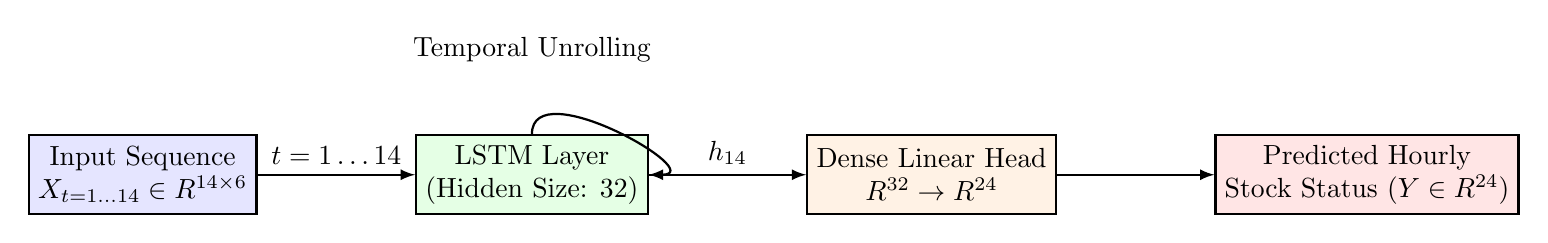
\begin{tikzpicture}[
        node distance=1.5cm and 2cm,
        box/.style={rectangle, draw, thick, minimum width=2.5cm, minimum height=1cm, align=center},
        arrow/.style={-latex, thick}
    ]
    % Nodes
    \node[box, fill=blue!10] (input) {Input Sequence \\ $X_{t=1 \dots 14} \in \mathbb{R}^{14 \times 6}$};
    \node[box, fill=green!10, right=of input] (lstm) {LSTM Layer \\ (Hidden Size: 32)};
    \node[box, fill=orange!10, right=of lstm] (dense) {Dense Linear Head \\ $\mathbb{R}^{32} \rightarrow \mathbb{R}^{24}$};
    \node[box, fill=red!10, right=of dense] (output) {Predicted Hourly \\ Stock Status ($Y \in \mathbb{R}^{24}$)};
    
    % Edges
    \draw[arrow] (input) -- node[above] {$t=1 \dots 14$} (lstm);
    \draw[arrow] (lstm) -- node[above] {$h_{14}$} (dense);
    \draw[arrow] (dense) -- (output);
    
    % Internal LSTM loop indication
    \draw[-latex, thick] (lstm.north) .. controls +(up:0.8cm) and +(right:0.8cm) .. (lstm.east);
    \node[above=0.8cm of lstm] {Temporal Unrolling};
    \end{tikzpicture}
    }
    \caption{The Canonical LSTM processing pipeline for 24-hour stockout prediction.}
    \label{fig:canonical_lstm}
\end{figure}

This Canonical LSTM was much faster (only 19,992 parameters) and slightly more accurate (0.7880 F1-Score). However, it still had a flaw: it forced the LSTM gates to track crazy demand spikes and actual physical inventory limits inside the exact same hidden state $h_t$, which confused the model.

\subsection{Baseline Transformers}
Because everyone uses Transformers nowadays, our team also tested some heavy Transformer models, specifically PatchTST \cite{nie2023patchtst} and Temporal Fusion Transformers (TFT) \cite{lim2021tft}. Even though they were massive (over 280,000 parameters), they actually did worse than our basic LSTM, getting F1-Scores around 0.7540 to 0.7685. Transformers are built to look at everything at once, which didn't fit well with our short 14-day history where physical stock goes down step-by-step. They were just too big for the job.

\section{Figuring Out Feature Importance}

Early on, our team wondered if we really needed all 13 features the dataset provided. Sometimes giving a model too much messy data just confuses it (which is probably why the Transformers failed). To fix this scientifically, we used a technique called Integrated Gradients (IG) \cite{sundararajan2017ig} to show us exactly what the model was paying attention to over the 14 days.

\begin{figure}[!htbp]
    \centering
    
\includegraphics[width=0.75\textwidth]{../btp-repo/docs/images/ig_heatmap.png}
    \caption{Integrated Gradients Heatmap revealing the disproportionate importance of recent inventory signals compared to historical static features.}
    \label{fig:ig_heatmap}
\end{figure}

As shown in Figure \ref{fig:ig_heatmap}, this test showed us two really important things that changed how we built the rest of our models:
\begin{enumerate}
    \item \textbf{Recent Data is King:} The data from the last two days ($t=13$ and $t=14$) was way more important than what happened two weeks ago.
    \item \textbf{Inventory Beats Demand:} Hard numbers about how much stock is left (like \texttt{stock\_hour6\_22\_cnt}) were far more useful than messy data about past sales or discounts.
\end{enumerate}

Based on this, our team threw out the bad data and kept only 6 essential features, giving our models a much cleaner signal to learn from.

\section{Building Our Custom LSTMs}

Armed with just the best features, our team started building a custom model piece-by-piece. We tested different structural setups to see what actually improved predictions. Table \ref{tab:rnn_variations} shows the steps we took.

\begin{table}[!htbp]
\centering
\caption{Systematic Progression of Recurrent Architectural Variations}
\label{tab:rnn_variations}
\begin{tabular}{llrr}
\toprule
\textbf{Stage} & \textbf{Architecture} & \textbf{Parameters} & \textbf{F1-Score} \\
\midrule
1 & Baseline SimpleRNN (h=64) & 14,744 & 0.7750 \\
2 & Dual-Stream SimpleRNN & 5,016 & 0.7782 \\
3 & Baseline Vanilla LSTM (h=96) & 44,952 & 0.7852 \\
4 & Feature-Reduced Canonical LSTM (h=32) & 19,992 & 0.7880 \\
5 & \textbf{Dual-Stream Inventory Shortcut LSTM} & \textbf{4,600} & \textbf{0.7941} \\
\bottomrule
\end{tabular}
\end{table}

\subsection{Our Final Custom LSTM: Dual-Stream Inventory Shortcut}

To fix the confusion happening inside the Canonical LSTM, we built our final custom model: the \textbf{Dual-Stream Inventory Shortcut LSTM}. 

We split the 6 good features into two groups: 4 features for Demand, and 2 features for Inventory. We gave each group its own separate LSTM to process. On top of that, because our heatmap showed that the very last day's inventory is the most important thing, we added a special "Shortcut." This shortcut takes the inventory numbers from Day 14 and sends them straight to the final output, completely bypassing the LSTMs. This guarantees that the LSTM never accidentally "forgets" the most important data.

\begin{figure}[!htbp]
    \centering
    \resizebox{\textwidth}{!}{
    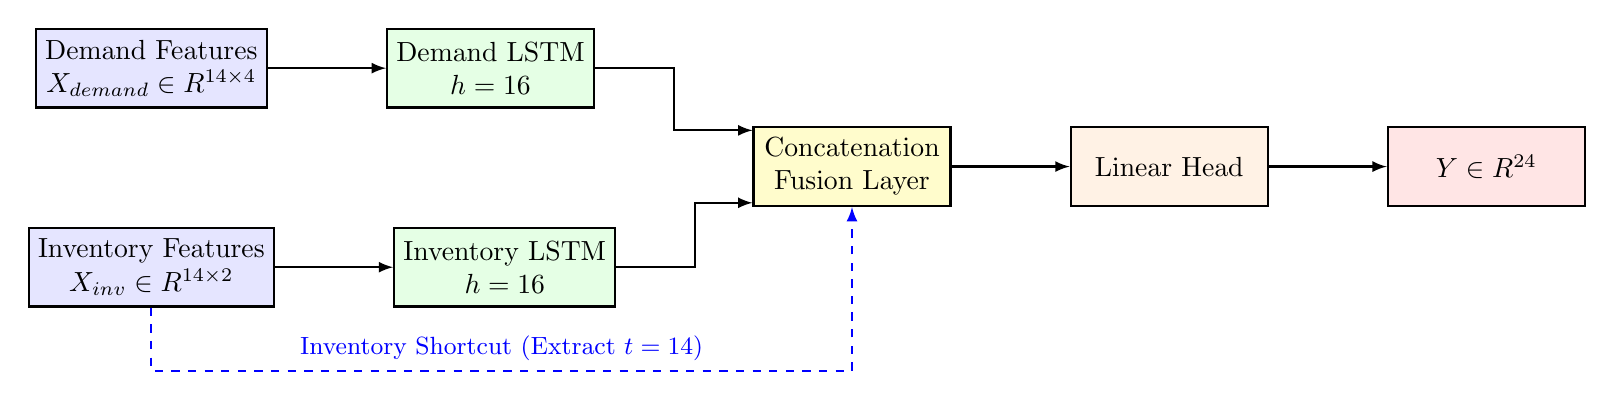
\begin{tikzpicture}[
        node distance=1.5cm and 1cm,
        box/.style={rectangle, draw, thick, minimum width=2.5cm, minimum height=1cm, align=center},
        arrow/.style={-latex, thick}
    ]
    % Inputs
    \node[box, fill=blue!10] (demand_in) {Demand Features \\ $X_{demand} \in \mathbb{R}^{14 \times 4}$};
    \node[box, fill=blue!10, below=1.5cm of demand_in] (inv_in) {Inventory Features \\ $X_{inv} \in \mathbb{R}^{14 \times 2}$};
    
    % LSTMs
    \node[box, fill=green!10, right=1.5cm of demand_in] (demand_lstm) {Demand LSTM \\ $h = 16$};
    \node[box, fill=green!10, right=1.5cm of inv_in] (inv_lstm) {Inventory LSTM \\ $h = 16$};
    
    % Concat and Output
    \node[box, fill=yellow!20, right=2cm of demand_lstm, yshift=-1.25cm] (concat) {Concatenation \\ Fusion Layer};
    \node[box, fill=orange!10, right=1.5cm of concat] (dense) {Linear Head};
    \node[box, fill=red!10, right=1.5cm of dense] (output) {$Y \in \mathbb{R}^{24}$};
    
    % Standard Paths
    \draw[arrow] (demand_in) -- (demand_lstm);
    \draw[arrow] (inv_in) -- (inv_lstm);
    \draw[arrow] (demand_lstm.east) -- ++(1,0) |- (concat.160);
    \draw[arrow] (inv_lstm.east) -- ++(1,0) |- (concat.200);
    
    % Shortcut Path
    \draw[arrow, dashed, thick, blue] (inv_in.south) -- ++(0,-0.8) -| node[pos=0.25, above, text=blue, font=\small] {Inventory Shortcut (Extract $t=14$)} (concat.south);
    
    % Final Paths
    \draw[arrow] (concat) -- (dense);
    \draw[arrow] (dense) -- (output);
    \end{tikzpicture}
    }
    \caption{The Dual-Stream Inventory Shortcut LSTM Architecture. Notice the dashed shortcut preserving the $t=14$ state.}
    \label{fig:dual_stream_lstm}
\end{figure}

This new design dropped the parameter count all the way down to just 4,600, but pushed our F1-Score up to 0.7941, making it our best recurrent model by far.

\section{DLinear (Decomposition Linear) Architectures}

After doing everything we could with LSTMs, our team wanted to see if newer Decomposition Linear (DLinear) models could do better. According to Zeng et al. (2023) \cite{zeng2023dlinear}, these simple, single-layer models that split time-series data into Trends and Seasons can sometimes beat complex deep learning models because they are simpler and don't get stuck trying to remember long sequences.

\subsection{Standard DLinear}

Standard DLinear takes the input data $X$ and splits it into a Trend piece ($X_{trend}$, found by averaging recent data) and a Seasonal piece ($X_{seasonal}$, found by subtracting the Trend from the original). The math looks like this:

\begin{align}
    X_{trend} &= \text{AvgPool1D}(X) \\
    X_{seasonal} &= X - X_{trend}
\end{align}

Then, it just uses standard linear layers ($W_{trend}, W_{seasonal}$) to map these pieces directly to the 24-hour prediction. It is very fast and easy to understand:

\begin{equation}
    Y_{pred} = (W_{trend} \cdot X_{trend}) + (W_{seasonal} \cdot X_{seasonal})
\end{equation}

\begin{figure}[!htbp]
    \centering
    \resizebox{0.9\textwidth}{!}{
    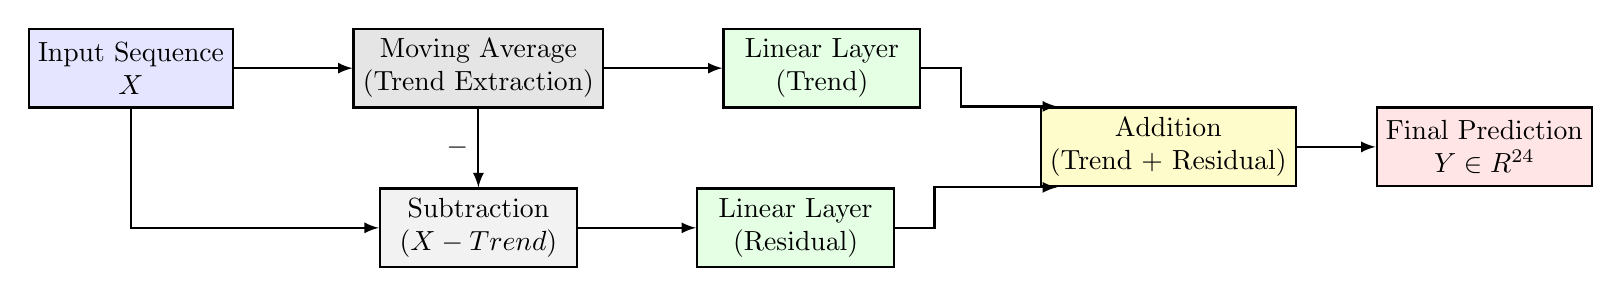
\begin{tikzpicture}[
        node distance=1cm and 1.5cm,
        box/.style={rectangle, draw, thick, minimum width=2.5cm, minimum height=1cm, align=center},
        arrow/.style={-latex, thick}
    ]
    % Input
    \node[box, fill=blue!10] (input) {Input Sequence \\ $X$};
    
    % Decomposition
    \node[box, fill=gray!20, right=1.5cm of input] (ma) {Moving Average \\ (Trend Extraction)};
    \node[box, fill=gray!10, below=1cm of ma] (residual) {Subtraction \\ ($X - Trend$)};
    
    % Linear Layers
    \node[box, fill=green!10, right=1.5cm of ma] (linear_trend) {Linear Layer \\ (Trend)};
    \node[box, fill=green!10, right=1.5cm of residual] (linear_res) {Linear Layer \\ (Residual)};
    
    % Output
    \node[box, fill=yellow!20, right=1.5cm of linear_trend, yshift=-1cm] (add) {Addition \\ (Trend + Residual)};
    \node[box, fill=red!10, right=1cm of add] (output) {Final Prediction \\ $Y \in \mathbb{R}^{24}$};
    
    % Edges
    \draw[arrow] (input) -- (ma);
    \draw[arrow] (input) |- (residual);
    \draw[arrow] (ma) -- node[left] {$-$} (residual);
    \draw[arrow] (ma) -- (linear_trend);
    \draw[arrow] (residual) -- (linear_res);
    \draw[arrow] (linear_trend.east) -- ++(0.5,0) |- (add.160);
    \draw[arrow] (linear_res.east) -- ++(0.5,0) |- (add.200);
    \draw[arrow] (add) -- (output);
    \end{tikzpicture}
    }
    \caption{The Standard DLinear Architecture. Trend and residual mapped via independent linear layers.}
    \label{fig:dlinear_arch}
\end{figure}

\subsection{Multi-Kernel DLinear}

To make DLinear work even better for the crazy ups and downs of grocery shopping, our team built the \textbf{Multi-Kernel DLinear}. Instead of just doing one average to find the trend, this model runs multiple averages at the same time (like $k=3, 5, 7$) to catch both sudden panic-buying and smooth weekly habits. It groups all these trends together like this:

\begin{equation}
    X_{trend} = \text{Concat}(\text{AvgPool1D}_{k=3}(X), \text{AvgPool1D}_{k=5}(X), \text{AvgPool1D}_{k=7}(X))
\end{equation}

\begin{figure}[!htbp]
    \centering
    \resizebox{0.8\textwidth}{!}{
    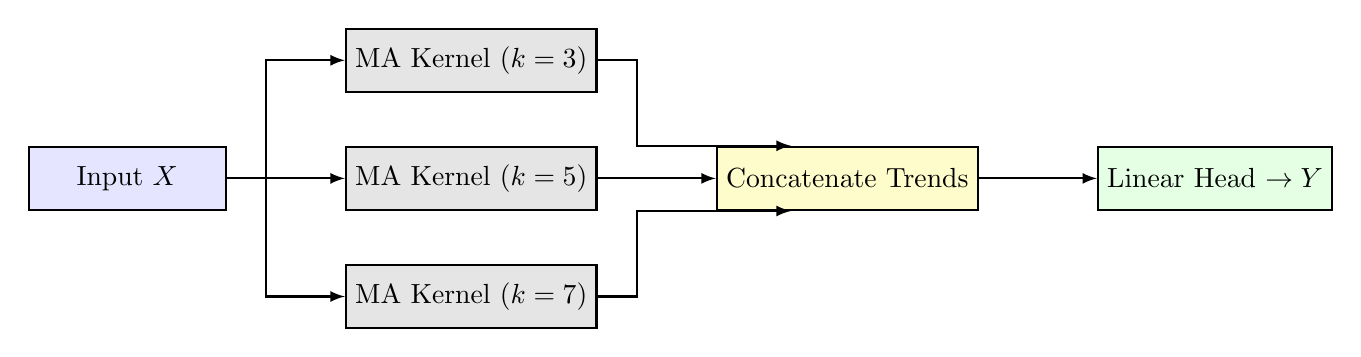
\begin{tikzpicture}[
        node distance=0.8cm and 1cm,
        box/.style={rectangle, draw, thick, minimum width=2.5cm, minimum height=0.8cm, align=center},
        arrow/.style={-latex, thick}
    ]
    % Input
    \node[box, fill=blue!10] (input) {Input $X$};
    
    % Kernels
    \node[box, fill=gray!20, right=1.5cm of input, yshift=1.5cm] (ma3) {MA Kernel ($k=3$)};
    \node[box, fill=gray!20, right=1.5cm of input] (ma5) {MA Kernel ($k=5$)};
    \node[box, fill=gray!20, right=1.5cm of input, yshift=-1.5cm] (ma7) {MA Kernel ($k=7$)};
    
    % Concat
    \node[box, fill=yellow!20, right=1.5cm of ma5] (concat) {Concatenate Trends};
    
    % Linear
    \node[box, fill=green!10, right=1.5cm of concat] (linear) {Linear Head $\rightarrow Y$};
    
    % Edges
    \draw[arrow] (input.east) -- ++(0.5,0) |- (ma3.west);
    \draw[arrow] (input) -- (ma5);
    \draw[arrow] (input.east) -- ++(0.5,0) |- (ma7.west);
    \draw[arrow] (ma3.east) -- ++(0.5,0) |- (concat.150);
    \draw[arrow] (ma5) -- (concat);
    \draw[arrow] (ma7.east) -- ++(0.5,0) |- (concat.210);
    \draw[arrow] (concat) -- (linear);
    \end{tikzpicture}
    }
    \caption{The Multi-Kernel DLinear extraction phase. Multiple kernels capture volatility at different frequencies.}
    \label{fig:multi_kernel_dlinear}
\end{figure}
\label{chap:methodology}
\clearpage
\thispagestyle{empty}
\newpage

\chapter{Tasks Completed}
\label{chap:tasks}

To achieve the final deployed model and comprehensively explore the structural challenges of high-frequency retail forecasting, the following tasks were systematically completed over a strict three-month timeline:

\begin{enumerate}
    \item \textbf{Month 1: Initial Research and Baseline Implementation} 
    \begin{itemize}
        \item Researched classical C1 supply and backorder forecasting methodologies.
        \item Processed the FreshRetailNet-50K dataset and structured it for basic classification.
        \item Built and trained the Vanilla RNN and Vanilla LSTM architectures, establishing the primary performance baselines (44K parameters, 0.785 F1-Score).
    \end{itemize}
    
    \item \textbf{Month 2: Feature Explainability and Recurrent Engineering}
    \begin{itemize}
        \item Utilized ML Explainability (Integrated Gradients) to aggressively prune the dataset down to 6 critical features, drastically reducing model noise.
        \item Designed the Dual-Stream processing pipeline to structurally isolate noisy demand variables from physical inventory variables.
        \item Finalized the \textit{Dual-Stream Inventory Shortcut LSTM}, successfully reducing parameters to 4,600 while boosting performance beyond the 44K-parameter baseline.
    \end{itemize}
    
    \item \textbf{Month 3: Linear Benchmarking and Final Evaluation}
    \begin{itemize}
        \item Developed a strict, standardized Top-15 holdout validation framework incorporating Focal Loss and dynamic threshold scanning.
        \item Engineered and benchmarked the \textit{Multi-Kernel DLinear} to capture both rapid retail volatility and longer multi-day trends.
        \item Generated all quantitative metrics, boxplots, and loss trajectory graphs to definitively prove the superiority of the Multi-Kernel DLinear model, culminating in the compilation of this final thesis report.
    \end{itemize}
\end{enumerate}
\label{chap:tasks}
\clearpage
\thispagestyle{empty}
\newpage

\chapter{Results and Conclusion}
\label{chap:results}

As our project went on, we knew we had to compare our custom LSTM models against the newest linear models to see which was truly better. This chapter explains how we tested everything fairly, shows our final numbers, and gives our overall conclusion.

\section{Standardized Evaluation Framework}

To make sure we were comparing apples to apples, our team set up a very strict testing process. This stopped any model from looking better just because of lucky guesses or messy data:

\begin{itemize}
    \item \textbf{Dataset Scope:} We only tested the top 15 busiest store-product combinations. This stopped the models from learning useless patterns from items that never sell anyway.
    \item \textbf{Holdout Strategy:} We used a strict timeline split. We hid the last 15 days of the dataset from the models completely, and only used those days for the final test.
    \item \textbf{Optimization:} In retail, stockouts don't happen as often as regular sales. To fix this imbalance, we trained the models using \textbf{Focal Loss} instead of standard Binary Cross-Entropy. The Focal Loss is defined mathematically as:
    \begin{equation}
        FL(p_t) = -\alpha_t (1 - p_t)^\gamma \log(p_t)
    \end{equation}
    where $p_t$ is the model's estimated probability for the stockout class. We configured the focusing parameter $\gamma = 2.0$ and the balancing factor $\alpha = 0.5$.
    \item \textbf{Dynamic Thresholding:} Instead of just picking a standard 50/50 cutoff for predictions, we had the computer scan all cutoffs from 10\% to 90\% on a practice set to find the perfect spot that maximized the F1-Score.
\end{itemize}

\section{Final Empirical Results}

We tested our main recurrent models against a few versions of the DLinear architecture (which we talked about in Chapter 4). You can see the final scores and how big each model is in Table \ref{tab:final_variants}.

\begin{table}[!htbp]
\centering
\caption{Performance Comparison of Final Evaluated Architectures}
\label{tab:final_variants}
\begin{tabular}{lrr}
\toprule
\textbf{Architecture} & \textbf{Parameters} & \textbf{Hour-Level F1} \\
\midrule
Vanilla LSTM & 44,952 & 0.7850 \\
Dual-Stream Inventory Shortcut LSTM & 4,600 & 0.7941 \\
Standard DLinear & 6,768 & 0.7932 \\
Hourly Slot-Specific DLinear & 6,744 & 0.8058 \\
\textbf{Multi-Kernel DLinear} & \textbf{13,539} & \textbf{0.8131} \\
\bottomrule
\end{tabular}
\end{table}

\begin{figure}[!htbp]
    \centering
    
\includegraphics[width=0.75\textwidth]{../btp-repo/docs/images/lstm_vs_dlinear_comparison.png}
    \caption{Final Empirical Comparison: The linear architectures systematically outperform the recurrent LSTM bounds.}
    \label{fig:final_comparison}
\end{figure}

The numbers clearly showed that the \textbf{Multi-Kernel DLinear} was the overall winner. It hit a peak F1-Score of \textbf{0.8131} while using only 13,539 parameters. It beat both our custom LSTM and all the basic baseline models (as you can see in Figure \ref{fig:final_comparison}). 

When we looked at all the different types of models we tried (Figure \ref{fig:family_comparison}), we saw that while the older recurrent models eventually stop improving, the linear models are faster, smaller, and just better at predicting exact hourly stockouts.

\begin{figure}[!htbp]
    \centering
    
\includegraphics[width=0.75\textwidth]{../btp-repo/docs/images/hourly_f1_vs_params_by_family.png}
    \caption{Broad comparison across model families, illustrating the parameter-efficiency dominance of DLinear variants on the FreshRetailNet-50K task.}
    \label{fig:family_comparison}
\end{figure}

\section{Conclusion}

This project took on the real-world problem of predicting hourly stockouts in fast-paced grocery delivery. By moving away from predicting daily totals and focusing on specific hour-by-hour predictions, our team tackled a problem that actually costs delivery apps a lot of customers.

Going through all these different models taught our team a few big lessons:

\begin{enumerate}
    \item \textbf{Good Features Matter Most:} Getting rid of bad data and focusing on a few strong features helped the models way more than just making the models bigger.
    \item \textbf{Routing the Data Helps:} When building LSTMs, separating the demand numbers from the inventory numbers, and taking a "shortcut" for the most recent day's data, stopped the model from forgetting the important stuff.
    \item \textbf{Linear Models Win Here:} In our strict testing, we proved that simple Decomposition Linear (DLinear) models are actually better for this specific short-term forecasting job than complex deep learning LSTMs.
\end{enumerate}

While our Dual-Stream Inventory Shortcut LSTM was our best idea for a recurrent model, the \textbf{Multi-Kernel DLinear} is the final model we recommend using in the real world. Because it doesn't have messy recurrent memory, it is very small (only 13,539 parameters) and fast. By running multiple averages at the same time, it easily handles the short 14-day history, catching both sudden panic-buying and smooth weekly trends to get the highest F1-Score of 0.8131. 

By predicting exactly which hour a shelf will empty, this tool can help grocery managers restock shelves before they run out. This means less spoiled food, less wasted money, and happier customers when they open the app to order.
\label{chap:results}
\clearpage
\thispagestyle{empty}
\newpage 

\addtocounter{page}{-1}

%************************************************ BEGIN REFERENCES **********************************************
\renewcommand{\bibname}{References}
\bibliographystyle{ieeetr}
\nocite{*}
\bibliography{references}
% \addcontentsline{toc}{chapter}{References} % Removed as per supervisor feedback
\clearpage
\appendix
%%%..........................................................................................................................................
%\fancychapter{Appendix}\label{Sunil_Appendix}
%\chapter{Appendix}\label{Sunil_Appendix}
%  \include{Chapters/Appendix/Appendix}
%\clearpage
%%..........................................................................................................................................
%\fancychapter{Cepstral Analysis}
%\label{app:lpc}
%\include{chapters/Appendix/CFA}
%\clearpage
%%..........................................................................................................................................
%\fancychapter{Linear Prediction Coefficients Computation}
%\label{app:sine}
%\include{chapters/Appendix/Appendix_lpc_V2}
%\clearpage
%%..........................................................................................................................................
%\fancychapter{Composite Objective Quality Measures}
%\label{app:cqm}
%\include{Chapters/Appendix/Appendix_cqm_V1}
%\clearpage
%%..........................................................................................................................................
%\fancychapter{MFCC Feature Extraction}
%\label{app:mfcc}
%\include{Chapters/Appendix/Appendix_mfcc_V1}
%\clearpage
%%..........................................................................................................................................
%\fancychapter{Gaussian Mixture Models}
%\label{app:gmm}
%\include{Chapters/Appendix/Appendix_gmm_V1}
%\clearpage
%..........................................................................................................................................
%\doublespacing
%\normalsize
%\pdfbookmark{Publications}{Publications}
%\fancyhead[LE]{\bfseries\small{List of Publications}}
%\fancyhead[RO]{\bfseries\small{List of Publications}}
%\pdfbookmark[1]{List of Publications}{los}
%\addstarredchapter{List of Publications}
%\include{FrontPages/publ}
%\clearpage

%% LIST OF SYMBOLS
%\fancyhead[LE]{\bfseries\small{List of Symbols}}
%\fancyhead[RO]{\bfseries\small{List of Symbols}}
%\pdfbookmark[1]{List of Symbols}{los}
%\addstarredchapter{List of Symbols}
%\include{FrontPages/Symbols}
%\clearpage
%******************************************************************************************************************************************************************

\end{document}
